\documentclass[11pt]{article}
\usepackage{microtype}
\usepackage{graphicx}
\usepackage{wrapfig}
\usepackage{dirtytalk}
\usepackage{url}
\usepackage{wrapfig}
\usepackage{color}
\usepackage{marvosym}
\usepackage{enumerate}
\usepackage{subfigure}
\usepackage{tikz}
\usepackage[fleqn]{amsmath}
\DeclareMathOperator*{\argmax}{arg\,max}
\DeclareMathOperator*{\argmin}{arg\,min}
\usepackage{amssymb}
\usepackage{hyperref}
\usepackage[many]{tcolorbox}
\usepackage{lipsum}
\usepackage{float}
\usepackage{trimclip}
\usepackage{listings}
\usepackage{environ}% http://ctan.org/pkg/environ
\usepackage{wasysym}
\usepackage{array}


\oddsidemargin 0mm
\evensidemargin 5mm
\topmargin -20mm
\textheight 240mm
\textwidth 160mm

\newcommand{\vwi}{{\bf w}_i}
\newcommand{\vw}{{\bf w}}
\newcommand{\vx}{{\bf x}}
\newcommand{\vy}{{\bf y}}
\newcommand{\vxi}{{\bf x}_i}
\newcommand{\yi}{y_i}
\newcommand{\vxj}{{\bf x}_j}
\newcommand{\vxn}{{\bf x}_n}
\newcommand{\yj}{y_j}
\newcommand{\ai}{\alpha_i}
\newcommand{\aj}{\alpha_j}
\newcommand{\X}{{\bf X}}
\newcommand{\Y}{{\bf Y}}
\newcommand{\vz}{{\bf z}}
\newcommand{\msigma}{{\bf \Sigma}}
\newcommand{\vmu}{{\bf \mu}}
\newcommand{\vmuk}{{\bf \mu}_k}
\newcommand{\msigmak}{{\bf \Sigma}_k}
\newcommand{\vmuj}{{\bf \mu}_j}
\newcommand{\msigmaj}{{\bf \Sigma}_j}
\newcommand{\pij}{\pi_j}
\newcommand{\pik}{\pi_k}
\newcommand{\D}{\mathcal{D}}
\newcommand{\el}{\mathcal{L}}
\newcommand{\N}{\mathcal{N}}
\newcommand{\vxij}{{\bf x}_{ij}}
\newcommand{\vt}{{\bf t}}
\newcommand{\yh}{\hat{y}}
\newcommand{\code}[1]{{\footnotesize \tt #1}}
\newcommand{\alphai}{\alpha_i}
\newcommand{\defeq}{\overset{\text{def}}{=}}
\renewcommand{\vec}[1]{\mathbf{#1}}
\newcommand{\indep}{\perp \!\!\! \perp}

\bgroup
\def\arraystretch{1.5}
\newcolumntype{x}[1]{>{\centering\arraybackslash\hspace{0pt}}p{#1}}
\newcolumntype{z}[1]{>{\centering\arraybackslash}m{#1}}

%Arguments are 1 - height, 2 - box title
\newtcolorbox{textanswerbox}[2]{%
 width=\textwidth,colback=white,colframe=blue!30!black,floatplacement=H,height=#1,title=#2,clip lower=true,before upper={\parindent0em}}

 \newtcolorbox{eqanswerbox}[1]{%
 width=#1,colback=white,colframe=black,floatplacement=H,height=3em,sharp corners=all,clip lower=true,before upper={\parindent0em}}

 %Arguments are 1 - height, 2 - box title
 \NewEnviron{answertext}[2]{
        \noindent
        \marginbox*{0pt 10pt}{
        \clipbox{0pt 0pt 0pt 0pt}{
        \begin{textanswerbox}{#1}{#2}
        \BODY
        \end{textanswerbox}
        }
        }
}

%Arguments are 1 - height, 2 - box title, 3 - column definition
 \NewEnviron{answertable}[3]{
        \noindent
        \marginbox*{0pt 10pt}{
        \clipbox{0pt 0pt 0pt 0pt}{
        \begin{textanswerbox}{#1}{#2}
                \vspace{-0.5cm}
                        \begin{table}[H]
                        \centering
                        \begin{tabular}{#3}
                                \BODY
                        \end{tabular}
                        \end{table}
        \end{textanswerbox}
        }
        }
}

 %Arguments are 1 - height, 2 - box title, 3 - title, 4- equation label, 5 - equation box width
 \NewEnviron{answerequation}[5]{
        \noindent
        \marginbox*{0pt 10pt}{
        \clipbox{0pt 0pt 0pt 0pt}{
        \begin{textanswerbox}{#1}{#2}
                \vspace{-0.5cm}
                        \begin{table}[H]
                        \centering
                \renewcommand{\arraystretch}{0.5}% Tighter

                        \begin{tabular}{#3}
                                #4 =	&
                        \clipbox{0pt 0pt 0pt 0pt}{

                        \begin{eqanswerbox}{#5}
                                $\BODY$
                        \end{eqanswerbox}
                        } \\
                        \end{tabular}
                        \end{table}

        \end{textanswerbox}
        }
        }
}

 %Arguments are 1 - height, 2 - box title
 \NewEnviron{answerderivation}[2]{
        \noindent
        \marginbox*{0pt 10pt}{
        \clipbox{0pt 0pt 0pt 0pt}{
        \begin{textanswerbox}{#1}{#2}
        \BODY
        \end{textanswerbox}
        }
        }
}

\newcommand{\Checked}{{\LARGE \XBox}}%
\newcommand{\Unchecked}{{\LARGE \Square}}%
\newcommand{\TextRequired}{{\textbf{Place Answer Here}}}%
\newcommand{\EquationRequired}{\textbf{Type Equation Here}}%


\newcommand{\answertextheight}{5cm}
\newcommand{\answertableheight}{4cm}
\newcommand{\answerequationheight}{2.5cm}
\newcommand{\answerderivationheight}{14cm}

\newcounter{QuestionCounter}
\newcounter{SubQuestionCounter}[QuestionCounter]
\setcounter{SubQuestionCounter}{1}

\newcommand{\subquestiontitle}{Question \theQuestionCounter.\theSubQuestionCounter~}
\newcommand{\newquestion}{\stepcounter{QuestionCounter}\setcounter{SubQuestionCounter}{1}\newpage}
\newcommand{\newsubquestion}{\stepcounter{SubQuestionCounter}}


\lstset{language=[LaTeX]TeX,basicstyle=\ttfamily\bf}

\pagestyle{myheadings}
\markboth{Homework 6}{Fall 2020 CS 475/675 Machine Learning: Homework 6}

\title{CS 475 Machine Learning: Homework 6\\
Graphical Models\\
Analytical Questions\\
\Large{Due: Dec 7, 2020, 11:59 pm US/Eastern}\\
50 Points Total \hspace{1cm} Version 1.1 (Updated Nov 30)}
\author{PARTNER1\_NAME (PARTNER1\_JHED), PARTER2\_NAME (PARTNER2\_JHED)}
\date{}

\begin{document}
\maketitle
\thispagestyle{headings}


\section*{Instructions }
We have provided this \LaTeX{} document for turning in this homework. We give you one or more boxes to answer each question.  The question to answer for each box will be noted in the title of the box.\\

{\bf Other than your name, do not type anything outside the boxes. Leave the rest of the document unchanged.}\\


\textbf{Do not change any formatting in this document, or we may be unable to
  grade your work. This includes, but is not limited to, the height of
  textboxes, font sizes, and the spacing of text and tables.  Additionally, do
  not add text outside of the answer boxes. Entering your answers are the only
  changes allowed.}\\


\textbf{We strongly recommend you review your answers in the generated PDF to
  ensure they appear correct. We will grade what appears in the answer boxes in
  the submitted PDF, NOT the original latex file.}

\pagebreak

%%%%%%%%%%%%%%%%%%%%%%%%%%%%%%%%%%%%%%%%%%%%%%%%%%%%%%%%%%%%%%%%%%%%%%%%%%%%%%%%
\newquestion
\section*{\arabic{QuestionCounter}) Expectation Maximization: Hidden Markov models to find genes}

DNA carries genetic information and is made of four bases A, C, G and T. Broadly, regions of the genome are either coding consisting of genes that encode the primary structure of proteins or non-coding. While the genome is made of roughly three million bases, protein coding genes only make up approximately 1\% of the genome. Biologists are interested in determining which regions of the genome correspond to protein coding genes since mutations in these regions can change the structure and hence function of proteins leading to pathological states. 
\begin{figure}[h]
    \centering
    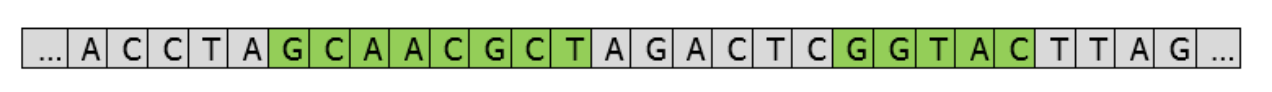
\includegraphics[width=1.0\textwidth]{genome.png}
    \caption{Example of DNA sub-sequence with genes shown in green}
    \label{Fig 1}
\end{figure}
\newline
In general, the observed frequency of different bases is different between the coding and the non-coding regions of the genome. For instance, C and G are found more often in protein coding regions. These statistical patterns can be exploited to identify regions corresponding to genes using Hidden Markov models. These models take as input the observed sequence of bases and includes latent binary hidden variables that encode whether a particular region is protein coding or not. When formulated in this manner, the observations and the latent variable are discrete and can only occupy finite states. 
\newline
\newline
Experimentally, different sequencing methods are employed to \say{read} the genome. One such method is nanopore sequencing which uses a protein nanopore set in an electrically resistant polymer membrane. An ionic current is passed through the pore by setting a voltage across this membrane, and as different bases pass through the pore, they result in different values of the current measured (Fig 2). Here, the observations are not discrete, rather the observed current values can be modeled using a Gaussian mixture model with four components corresponding to each base.  
\begin{figure}[h]
    \centering
    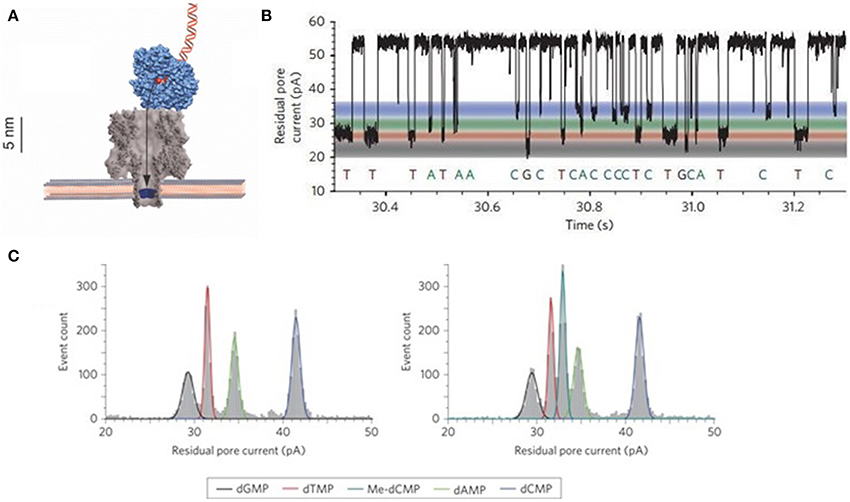
\includegraphics[width=1.0\textwidth]{nanopore.jpg}
    \caption{(A) Schematic representation of nanopore sequencing, (B) Observed current as the strand is read, (C) The distribution of residual pore current for different bases}
    \label{Fig 2}
\end{figure}
\newline
\newline
We would like to identify whether a particular region of the genome is protein coding or not based on observing the pore residual current. Further, we would like to obtain the most probable sequence of bases given a certain current observation. The model we will use for this is called tied-mixture HMM. 
\newline
\newline
For a DNA sequence of length T, $z_t$ determines the region type of the $t$-th base and $x_t$ is the electrical signal for the $t$-th base. Finally, the value of the $t$-th base is given by $y_t$ which is called the mixture variable of the model. We specify our model as below 
\begin{align}
    p(z_1 = 1) = a_1 \\
    p(z_t = j | z_{t-1} = i) = a_{ij} \qquad i = 1, 2 \qquad j = 1, 2\\
    p(y_t = j | z_t = 1) = b_{ij} \qquad i = 1, 2 \qquad j = 1, 2, 3, 4\\
    p(x_t | y_t) = \prod_{i = 1}^4 \mathcal{N}(\mu_i, \sigma_i)^{\mathbb{I}(y_t = i)}
\end{align}
The parameters in our model are therefore 
\begin{align*}
    a_1 &: \text{The initial probability of $z_1=1$}\\
    a_{i,j} &: \text{The transition probability of $z_{t}$ to $z_{t +1}$} \\
    b_{i,j} &: \text{The probability of a particular base given that a region is protein coding} \\
    \mu_i &: \text{Mean residual current for a given base i} \\
    \sigma_i &: \text{Standard deviation of residual current for a given base i}
\end{align*}
We are given $S$ sequences ${\{x_1^s, \dots, x_T^s\}_{s=1}^S}$. Therefore the complete data likelihood is given by, 
\begin{align}
     p(\mathcal{D}) = \prod_{s=1}^S p(x^s_1|y^s_1, \vec{\mu}, \vec{\sigma})p(y^s_1|z^s_1, \vec{b})p(z^s_1|a_1) \prod_{t=2}^T p(x^s_t|y^s_t, \vec{\mu}, \vec{\sigma})p(y^s_t|z^s_t, \vec{b})p(z^s_t | z^s_{t-1}, \vec{a})
\end{align}
\begin{align}
        \text{log p}(\mathcal{D}) = \sum_{s=1}^S &\Bigg[ \text{log p}(x^s_1|y^s_1, \vec{\mu}, \vec{\sigma}) +  \text{log p}(y^s_1|z^s_1, \vec{b}) + \text{log p}(z^s_1 | a_1) \nonumber\\
    &+ \sum_{t=2}^T \text{log p}(x^s_t|y^s_t, \vec{\mu}, \vec{\sigma}) +  \text{log p}(y^s_t|z^s_t, \vec{b}) \nonumber\\
    &+ \text{log p}(z^s_t | z^s_{t-1}, \vec{a})\Bigg]
\end{align}
\begin{enumerate}[{(a)}]
\item In the E-step, we compute the posterior of the latent variables given the data, and set the $q(.)$ distribution to the posterior. Using Bayes rule compute $p(\vec{y}, \vec{z}|\vec{x}, \Theta^{old})$. Hint: $\vec{x} \indep \vec{z} | \vec{y}$ Propose an algorithm to compute the posterior exactly (How will you compute the marginal in the denominator?)
\newline
\begin{answertext}{9cm}{}
    
\end{answertext} 
\item In the M-step, we would like to maximize the $Q(\Theta \mid \Theta^{old})$ which is the expectation of the complete data log likelihood with respect to the posterior of the latent variables. Therefore,
\begin{align}
    Q(\Theta \mid \Theta^{old}) &= \text{E}[\text{log p}(\vec{x}, \vec{y}, \vec{z} | \Theta) | \vec{x}, \Theta^{old}] \\ 
    &= \sum_{\mathcal{Y},\mathcal{Z}} p(\vec{y}, \vec{z}|\vec{x}, \Theta^{old}) \text{log p}(\vec{x}, \vec{y}, \vec{z} | \Theta)
\end{align} Assuming you have access $p(\vec{y}, \vec{z}|\vec{x}, \Theta^{old})$ from part (a), write out the expression for $Q(\theta \mid \theta^\text{old})$ in terms of the components of $\theta$: $a_1, a_{i, j}, b_{i,j}, \mu_i,$ and $\sigma_i$.
\newline
\begin{answertext}{9cm}{}
    
\end{answertext}
\item Finally, we can compute the gradients of the $Q(\Theta \mid \Theta^{old})$ w.r.t our parameters to derive the updates. Derive an expression for $\mu^{n + 1}$ in terms of the data and the parameters from the previous iteration $\Theta^{n}$. 
\newline
\begin{answertext}{9cm}{}
    
\end{answertext}

Suppose you trained your HMM using EM on a dataset and obtained the following transition and emission probabilities. 
\begin{align}
    p(z_1 = \textbf{P}) = 0.5 \nonumber
\end{align}
\begin{tabular}{cccc}
                             & \multicolumn{3}{c}{Next}                                                       \\ \cline{2-4} 
\multicolumn{1}{c|}{Current} & P                        & N                        & \multicolumn{1}{c|}{End} \\ \hline
\multicolumn{1}{|c|}{Start} & \multicolumn{1}{c|}{0.5} & \multicolumn{1}{c|}{0.5} & \multicolumn{1}{c|}{0} \\
\multicolumn{1}{|c|}{P}      & \multicolumn{1}{c|}{0.7} & \multicolumn{1}{c|}{0.2} & \multicolumn{1}{c|}{0.1} \\
\multicolumn{1}{|c|}{N}      & \multicolumn{1}{c|}{0.1} & \multicolumn{1}{c|}{0.8} & \multicolumn{1}{c|}{0.1} \\ \hline
\end{tabular}
\qquad \qquad \qquad \qquad
\begin{tabular}{c|cccc|}
\cline{2-5}
                            & \multicolumn{4}{c|}{Base}                                                            \\ \hline
\multicolumn{1}{|c|}{State} & A                        & C                        & G                        & T   \\ \hline
\multicolumn{1}{|c|}{P}     & \multicolumn{1}{c|}{0.2} & \multicolumn{1}{c|}{0.3} & \multicolumn{1}{c|}{0.3} & 0.2 \\ \cline{2-5} 
\multicolumn{1}{|c|}{N}     & \multicolumn{1}{c|}{0.3} & \multicolumn{1}{c|}{0.2} & \multicolumn{1}{c|}{0.2} & 0.3 \\ \hline
\end{tabular}
\newline
\newline
\newline
We will assume that we are provided with the nucleotide sequence and are required to predict the most probable path that generated the sequence. 
An example of an input sequence is \textbf{AGCTTAACG}. The latent variables $\vec{z}$ encode whether a particular base belongs to a protein coding region or not and $\vec{z} \in \{\textbf{P}, \textbf{N}\}$. The graphical model corresponding to this setup is shown below. 
\begin{figure}[h]
    \centering
    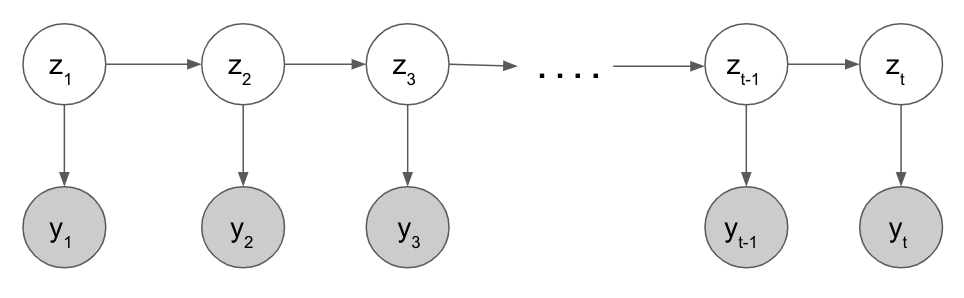
\includegraphics[width=0.6\textwidth]{HMM.png}
    \caption{$z_i$ refers to the latent state and $y_i$ is the observed base at the $i^{th}$ position}
    \label{Fig 3}
\end{figure}
\item We observe that the path P (states of latent variables z) given by \{\textbf{N N P P P P}\} produces the sequence S given by \{\textbf{G C T G G C}\}. What is the probability that the HMM described above produced sequence S by the path P?
    \newline
    \begin{answertext}{8cm}{}
    
    \end{answertext}
  \item We observe the sequence \{\textbf{G C T A A C}\} and we would like to determine the most likely path that produced this sequence and the probability associated with this path. To do this we can use max-product or in this case because we're working with a HMM, Viterbi decoding. Viterbi decoding relies on the following recursion by noting that the probability of the most probable path for the $t^{th}$ observation to be $i \in \{A, C, G, T\}$, given that it was in state $k \in \{P, N\}$ depends on the most probable path for the $(t-1)^{th}$ observation for base $j \in \{A, C, G, T\}$.
    \begin{align}
        \text{Probability of the most probable path} &= p_k(t = i) \nonumber \\
        &= e_k(i) \max_{s} [p_{s}(t - 1 = j) \cdot p_{sk}] \nonumber
    \end{align}
    Where $e_k(i)$ is the probability that base i is observed when the latent state is $k \in \{P, N\}$. Specify the most probable path and the associated probability below. Show your work. Hint: Refer to the \href{http://www.cs.jhu.edu/~jason/papers/#eisner-2002-tnlp}{\color{blue} ice cream and weather example} by Jason Eisner.
    \newline
    \begin{answertext}{3cm}{}
\end{answertext}
\begin{answertext}{15cm}{}
\end{answertext}
\end{enumerate}

% %%%%%%%%%%%%%%%%%%%%%%%%%%%%%%%%%%%%%%%%%%%%%%%%%%%%%%%%%%%%%%%%%%%%%%%%%%%%%%%%
\newquestion
\section*{\arabic{QuestionCounter}) Belief propagation in Factor graphs}
Recall, that we discussed for an undirected graphical model, the factorization of the joint probability distribution specified by a particular graph is not unique. One such factorization relies on the identification of maximal cliques. For a graph $G = {V, E}$, a complete subgraph $G''$ satisfies the condition $G'' = \{V' \subseteq \V, E' \subseteq E\}$ such that the nodes in $V'$ are fully interconnected. A (maximal) clique is a complete subgraph such that any $V'' \supset V'$ is not complete. A sub-clique is not necessarily a maximal clique. The maximal clique factorization can be used to convert an undirected graph to a factor graph. \newline
\begin{figure}[h]
    \centering
    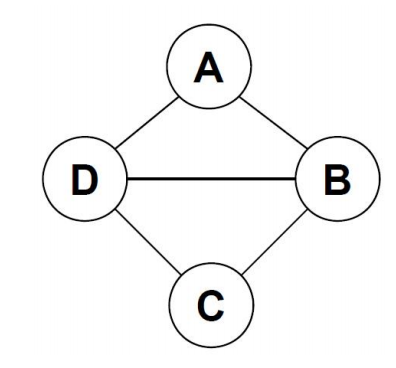
\includegraphics[width=0.2\textwidth]{maximal_cliques.png}
    \caption{The maximal cliques in this case are given by $\{A, B, D\}$ and $\{ B, C, D\}$}
    \label{Fig 3}
\end{figure}
    \begin{figure}[h]
    \centering
    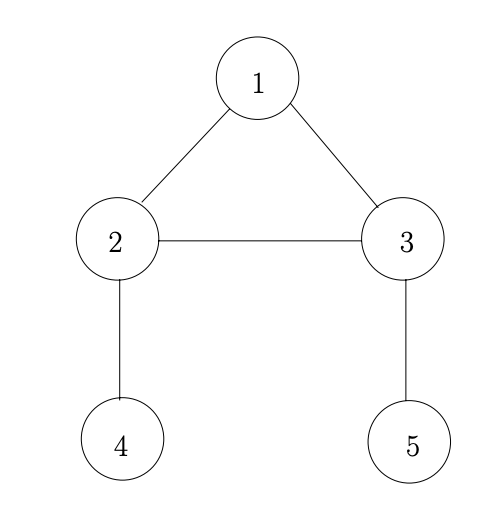
\includegraphics[width=0.3\textwidth]{undirected_graph.png}
    \caption{Undirected graph with 5 random variables}
    \label{Fig 4}
\end{figure}
\begin{enumerate}[{(a)}]
    \item Consider the undirected graph shown in Fig 5. Identify the maximal cliques and write a factor graph that represents the joint distribution of the product of the factors given by maximal cliques. In this example, why can we use factor graph message passing equations to compute the marginals but not sum product? Note: You can draw the graph using your favorite text/ slide editor and include as a .jpg (or whatever file format is easiest).
    \newline
\begin{answertext}{4cm}{}
    
\end{answertext}
\begin{answertext}{6cm}{}
    
\end{answertext}
\item For the factor graph that you obtained in part (a) write out all the messages that would be calculated by the sum product algorithm. Recall that in order for a factor or a node to pass messages, it should have received messages from all neighbors but one. Therefore begin with the message passed by the leaf nodes. Use $\psi_{i,j}(x_i, x_j)$ to denote the factors that are connected to nodes i, j and $\nu_{i \rightarrow f}(x_i)$ to denote a message passed from node i to factor f. Each variable is discrete with K classes. Write the messages in terms of factors and previous messages. If you write your messages as the full distribution over the K classes, you may also need to include K in your equations. 
\newline
\begin{answertext}{12.0cm}{}
    
\end{answertext}
\item Construct a new random variable given by $x_6 = \{x_1, x_2, x_3\}$, we group the three random variables $x_1, x_2, x_3$ into one. Now draw an undirected graph that captures the relationship between $x_6, x_4$ and $x_5$. Explain why the sum-product algorithm can be used to compute marginals now. Note: You can draw the graph using your favorite text/ slide editor and include as a .jpg (or whatever file format is easiest).
\newline
\begin{answertext}{8.5cm}{}
    
\end{answertext}
\item Write the sum product algorithm for graph you obtained in part (c). Note: $\psi_{5, 6}(x_5, x_6) = \psi_{5,6}(x_1, x_2, x_3, x_6)$. Compare the message passing equations that you obtained using sum product to the message passing you derived for the factor graph in (b). 
\newline
\begin{answertext}{9.5cm}{}
    
\end{answertext}

\item Taking the approach in (c) to the extreme, we can group all the variables in the graph to create a new random variable $x_7= \{x_1, x_2, x_3, x_4, x_5\}$. Assuming that we only care about the marginals of $x_1, x_2, x_3, x_4$ and $x_5$, why would we prefer the method proposed in part (c) to grouping all the variables, i.e. why might it be preferable to group a smaller number of variables together?
\newline
\begin{answertext}{7cm}{}
    
\end{answertext}
\end{enumerate}
% %%%%%%%%%%%%%%%%%%%%%%%%%%%%%%%%%%%%%%%%%%%%%%%%%%%%%%%%%%%%%%%%%%%%%%%%%%%%%%%%
\newquestion
\section*{\arabic{QuestionCounter}) Graphical modeling and inference}
Consider the biological model which is represented by the following directed graphical model. $G_i$ refers to the genotype of an individual. $G_i = 1$ if the individual has a healthy copy of the gene and $G_i = 2$ if the copy is unhealthy. $G_1$ is the genotype of the parent, while $G_2$ and $G_3$ correspond to the genotypes of the children. $X_i \in \mathbb{R}$ corresponds to the phenotype of interest, in this case BMI. Healthy individuals have $BMI \leq 25$, while a $BMI \geq 30$ is considered unhealthy. (We will make a simplifying assumption that it's not unhealthy to have a BMI value that is too low, although it is). We define the conditional probability distributions as follows. 
\begin{align}
    p(G_1) = [0.5, 0.5] \\
    p(G_2 |G_1) = \begin{pmatrix}
    0.8 & 0.2\\
    0.2 & 0.8\\
    \end{pmatrix} \\
    p(G_3 |G_1) = \begin{pmatrix}
    0.8 & 0.2\\
    0.2 & 0.8\\
    \end{pmatrix} \\
    p(X_i | G_i = 1) = \mathcal{N}(\X_i | \mu = 21, \sigma^2 = 3) \\
    p(X_i | G_i = 2) = \mathcal{N}(\X_i | \mu = 24, \sigma^2 = 3)
\end{align}
The meaning of the matrix for $p(G_2 = 1|G_1 = 1) = 0.8$ and $p(G_2 = 1|G_1 = 2) = 0.2$ etc.
\begin{figure}[h]
    \centering
    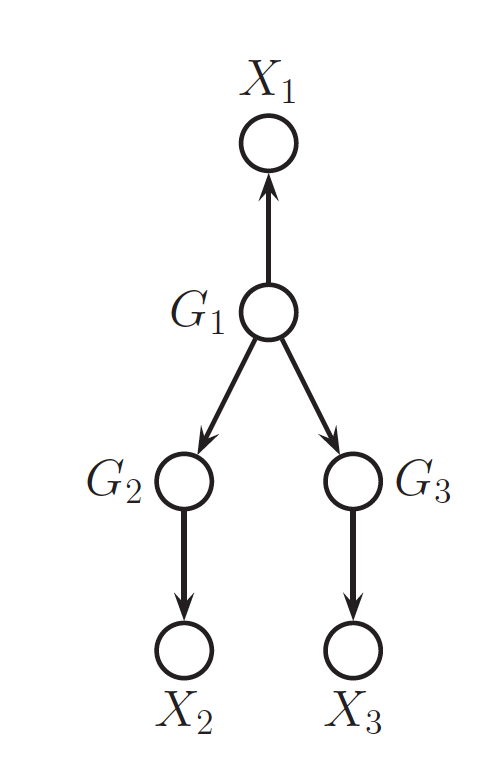
\includegraphics[width=0.2\textwidth]{inheritance.png}
    \caption{Directed graphical model explaining the relationship between the genotypes and phenotypic dependence on genotype}
    \label{Fig 3}
\end{figure}
\begin{enumerate}[{(a)}]
\item Suppose we observe $X_2 = 21$, and $X_1$ is unobserved, what is the posterior belief on $G_1$, i.e. $p(G_1| X_2 = 21)$? \newline
\begin{answertext}{5cm}{}
    
\end{answertext}
\item Now you observe that $X_2 = 21$ and $X_3 = 21$. What is $p(G_1|X_2, X_3)$? Explain how your answer is different from what you obtained in part (a)?
\newline
\begin{answertext}{7cm}{}
    
\end{answertext}
\item Now you observe that $X_2 = 21$ and $X_3 = 24$. What is $p(G_1|X_2, X_3)$? Compare to the answers you obtained in (a) and (b), are you more or less certain about the genotype of the parent when the children exhibit different phenotypes?
\newline
\begin{answertext}{6cm}{}
    
\end{answertext}
\end{enumerate}
\end{document}
